
\documentclass[a4paper, 12pt]{article}
\usepackage[utf8]{inputenc}
\usepackage[T1]{fontenc}
\usepackage[slovak]{babel}
\usepackage{geometry}
\usepackage{graphicx}
\usepackage{svg}
\usepackage{url}
\usepackage{listings}
\usepackage{xcolor}
\usepackage{amsmath}
\usepackage{amssymb}
\usepackage[hidelinks,breaklinks=true]{hyperref}
\usepackage{booktabs}

\def\UrlBreaks{\do\/\do-\do.\do=\do?\do\&}
\Urlmuskip=0mu plus 1mu
\usepackage{multirow}
\usepackage{float}
\usepackage{subcaption}

\geometry{a4paper, left=2.5cm, right=2.5cm, top=2.5cm, bottom=2.5cm}

\lstset{
    basicstyle=\ttfamily\small,
    breaklines=true,
    frame=single,
    numbers=left,
    numberstyle=\tiny,
    showstringspaces=false,
    commentstyle=\color{gray},
    keywordstyle=\color{blue},
    stringstyle=\color{red}
}

\title{Tímový projekt \\ Virtual Data Analyst \\ Inteligentný systém pre analýzu dát pomocou prirodzeného jazyka}
\author{Peter Muzslay, Janka Tarčákova, Jana Kampová, Jozef Guláš, Tamara Uhrinová}
\date{Akademický rok 2024/2025}

\begin{document}

\maketitle
\clearpage
\tableofcontents
\clearpage

\section{Úvod}

Projekt \textbf{Virtuálny dátový analytik} predstavuje moderný webový systém, ktorý umožňuje používateľom analyzovať dáta v~databázach pomocou prirodzeného jazyka. Využitím pokročilých techník spracovania prirodzeného jazyka (NLP) a~veľkých jazykových modelov (LLM) dokáže systém transformovať otázky v~bežnom jazyku na SQL dotazy, vykonať ich nad databázou a~následne vrátiť zrozumiteľné odpovede.

Hlavným cieľom projektu je demokratizácia prístupu k~dátovej analytike -- umožniť aj netechnickým používateľom efektívne získavať informácie z~databáz bez potreby znalosti SQL alebo iných programovacích jazykov.

\subsection{Motivácia}

V~súčasnej dobe je dátová analytika kľúčovým faktorom pri rozhodovaní v~mnohých oblastiach podnikania. Avšak tradičné nástroje pre prácu s~databázami vyžadujú:
\begin{itemize}
    \item Znalosť SQL jazyka
    \item Pochopenie štruktúry databázy
    \item Technické zručnosti pre interpretáciu výsledkov
\end{itemize}

Virtuálny dátový analytik tieto bariéry odstraňuje a~sprístupňuje dátovú analýzu širšiemu okruhu používateľov.

\subsection{Štruktúra projektu}

Projekt je rozdelený do nasledujúcich hlavných komponentov:

\begin{enumerate}
    \item \textbf{Frontend} -- Používateľské rozhranie (React + Vite)
    \item \textbf{Backend} -- Serverová aplikácia (FastAPI, Python)
    \item \textbf{GenAI Core} -- Jadro pre spracovanie prirodzeného jazyka (LLM)
    \item \textbf{Databázová vrstva} -- Pripojenie a~správa databáz
\end{enumerate}

\clearpage

\section{Riešený problém}

\subsection{Definícia problému}

Hlavný problém, ktorý projekt rieši, je \textbf{preklad prirodzeného jazyka na štruktúrované databázové dotazy} a~následná \textbf{interpretácia výsledkov} pre koncového používateľa.

Konkrétne výzvy zahŕňajú:
\begin{itemize}
    \item \textbf{Sémantické porozumenie} -- Pochopenie zámeru používateľa z~neformálnej otázky
    \item \textbf{Mapovanie na schému} -- Správne priradenie entít v~otázke k~tabuľkám a~stĺpcom databázy
    \item \textbf{Generovanie validného SQL} -- Syntakticky a~sémanticky správne dotazy
    \item \textbf{Bezpečnosť} -- Zabezpečenie len čítacích operácií (READ-ONLY)
    \item \textbf{Zrozumiteľná odpoveď} -- Sumarizácia výsledkov v~prirodzenom jazyku
\end{itemize}

\subsection{Príklad použitia}

\begin{table}[H]
\centering
\begin{tabular}{p{6cm}p{8cm}}
\toprule
\textbf{Vstup (používateľ)} & \textbf{Výstup (systém)} \\
\midrule
„Koľko objednávok bolo vytvorených v~novembri 2019?" & Vygenerovaný SQL dotaz, počet záznamov a~textová sumarizácia výsledkov \\
\midrule
„Aký je priemerný počet položiek na objednávku?" & Analytický výsledok s~vysvetlením \\
\midrule
„Ukáž mi top 10 produktov podľa predaja" & Zoradený zoznam s~popisom \\
\bottomrule
\end{tabular}
\caption{Príklady interakcie s~virtuálnym analytikom}
\end{table}

\clearpage

\section{Prístup a~metodológia}

\subsection{Výber technológií}

Pri návrhu systému sme zvolili nasledujúce technológie:

\begin{table}[H]
\centering
\begin{tabular}{llp{7cm}}
\toprule
\textbf{Komponent} & \textbf{Technológia} & \textbf{Zdôvodnenie} \\
\midrule
Frontend & React + Vite & Moderný, reaktívny framework s~rýchlym vývojovým prostredím \\
Backend & FastAPI (Python) & Asynchrónne API s~automatickou dokumentáciou \\
Databáza & PostgreSQL & Robustná open-source relačná databáza \\
LLM & GPT-4.1 / Gemini 2.5 & Najmodernejšie jazykové modely pre NLP úlohy \\
Cache & Redis & In-memory databáza pre rýchle ukladanie do vyrovnávacej pamäte \\
Kontajnerizácia & Docker & Konzistentné prostredie pre vývoj a~nasadenie \\
\bottomrule
\end{tabular}
\caption{Použité technológie a~ich zdôvodnenie}
\end{table}

\subsection{Architektúra GenAI Core}

Jadro systému pre spracovanie prirodzeného jazyka pozostáva z~troch hlavných komponentov:

\begin{enumerate}
    \item \textbf{Router (LLM)} -- Rozhoduje o~spôsobe spracovania dotazu
    \item \textbf{Query Generator} -- Generuje SQL dotazy z~prirodzeného jazyka
    \item \textbf{Response Summarizer} -- Sumarizuje výsledky pre používateľa
\end{enumerate}

\subsubsection{Query Generator}

Komponent využíva model \texttt{GPT-4.1} pre generovanie SQL dotazov. Systémový prompt definuje pravidlá:
\begin{itemize}
    \item Generovať \textbf{len SELECT} dotazy (read-only prístup)
    \item Nikdy nepoužívať INSERT, UPDATE, DELETE, DROP, CREATE a~iné modifikačné príkazy
    \item Vrátiť len čistý SQL dotaz bez vysvetlení
    \item Používať správnu PostgreSQL syntax
\end{itemize}

\subsubsection{Response Summarizer}

Komponent využíva model \texttt{Gemini 2.5 Flash} pre sumarizáciu výsledkov. Poskytuje:
\begin{itemize}
    \item Popis, čo dáta zobrazujú
    \item Zvýraznenie kľúčových poznatkov a~vzorcov
    \item Zmienku o~významných hodnotách alebo trendoch
    \item Zrozumiteľný text pre netechnických používateľov
\end{itemize}

\clearpage

\section{Architektúra systému}

\subsection{Vysokoúrovňová architektúra (High-Level)}

Systém je navrhnutý ako \textbf{trojvrstvová architektúra} s~jasne oddelenými zodpovednosťami:

\begin{figure}[H]
\centering
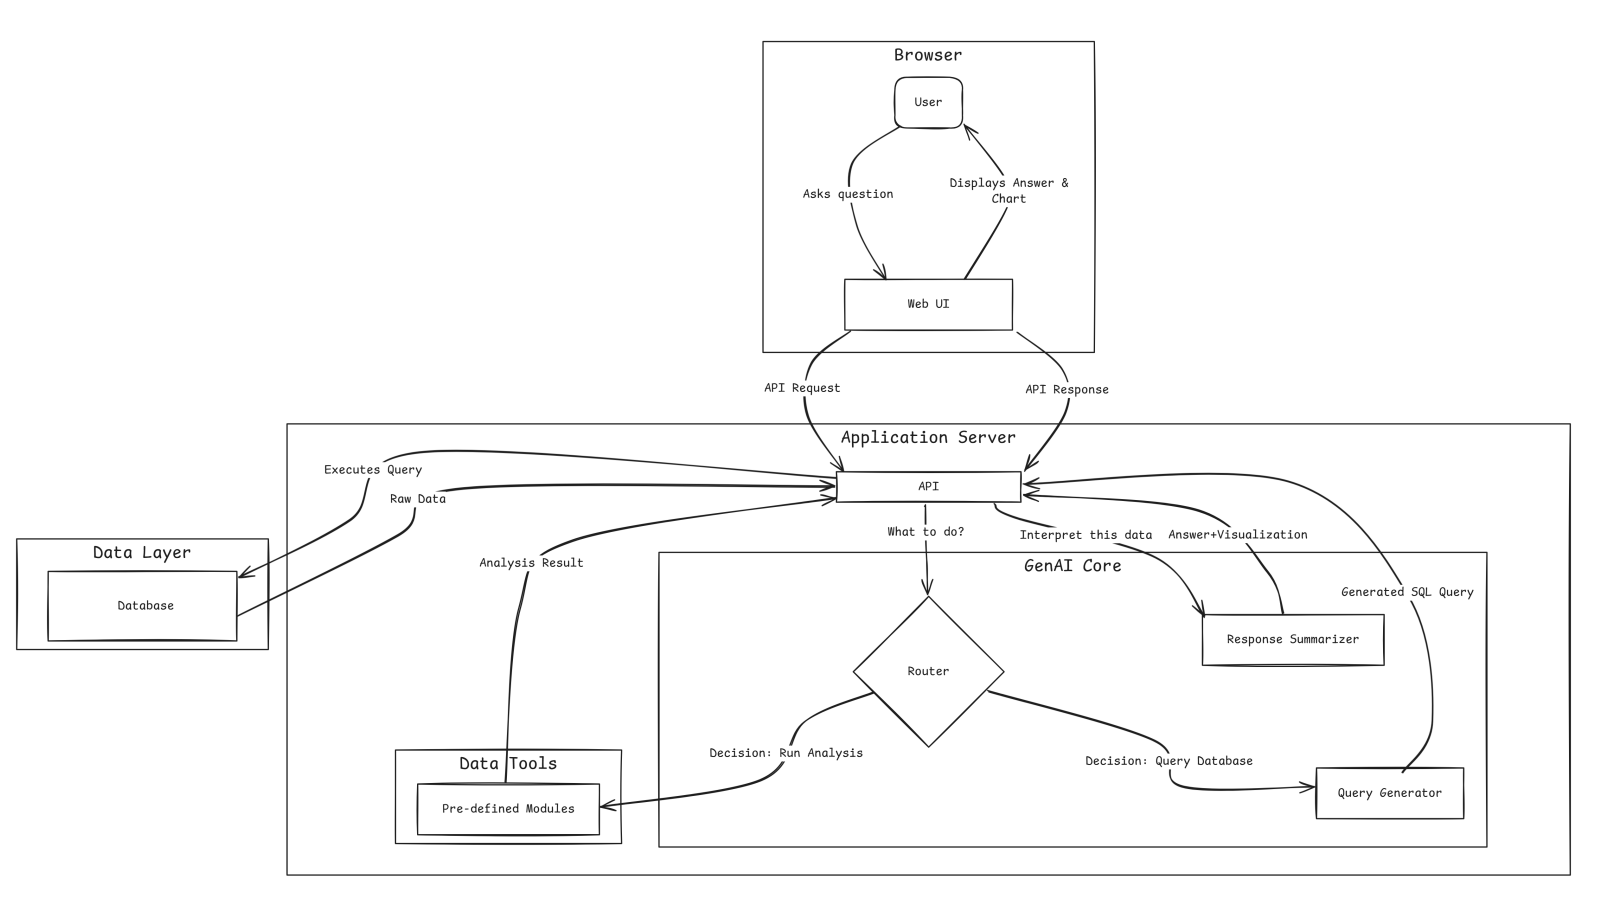
\includegraphics[width=0.95\textwidth]{high_level_VDA.png}
\caption{Vysokoúrovňová architektúra systému}
\end{figure}

\subsubsection{Tok dát (Data Flow)}

\begin{enumerate}
    \item Používateľ zadá otázku v~prirodzenom jazyku cez webové rozhranie
    \item Frontend odošle požiadavku na Backend API (\texttt{/api/ask})
    \item Backend získa schému databázy
    \item Query Generator (GPT-4.1) vygeneruje SQL dotaz
    \item Dotaz sa vykoná nad databázou (READ-ONLY)
    \item Response Summarizer (Gemini 2.5) vytvorí textovú sumarizáciu
    \item Odpoveď sa vráti používateľovi
\end{enumerate}

\clearpage

\subsection{Technická architektúra (Low-Level)}

\begin{figure}[H]
\centering
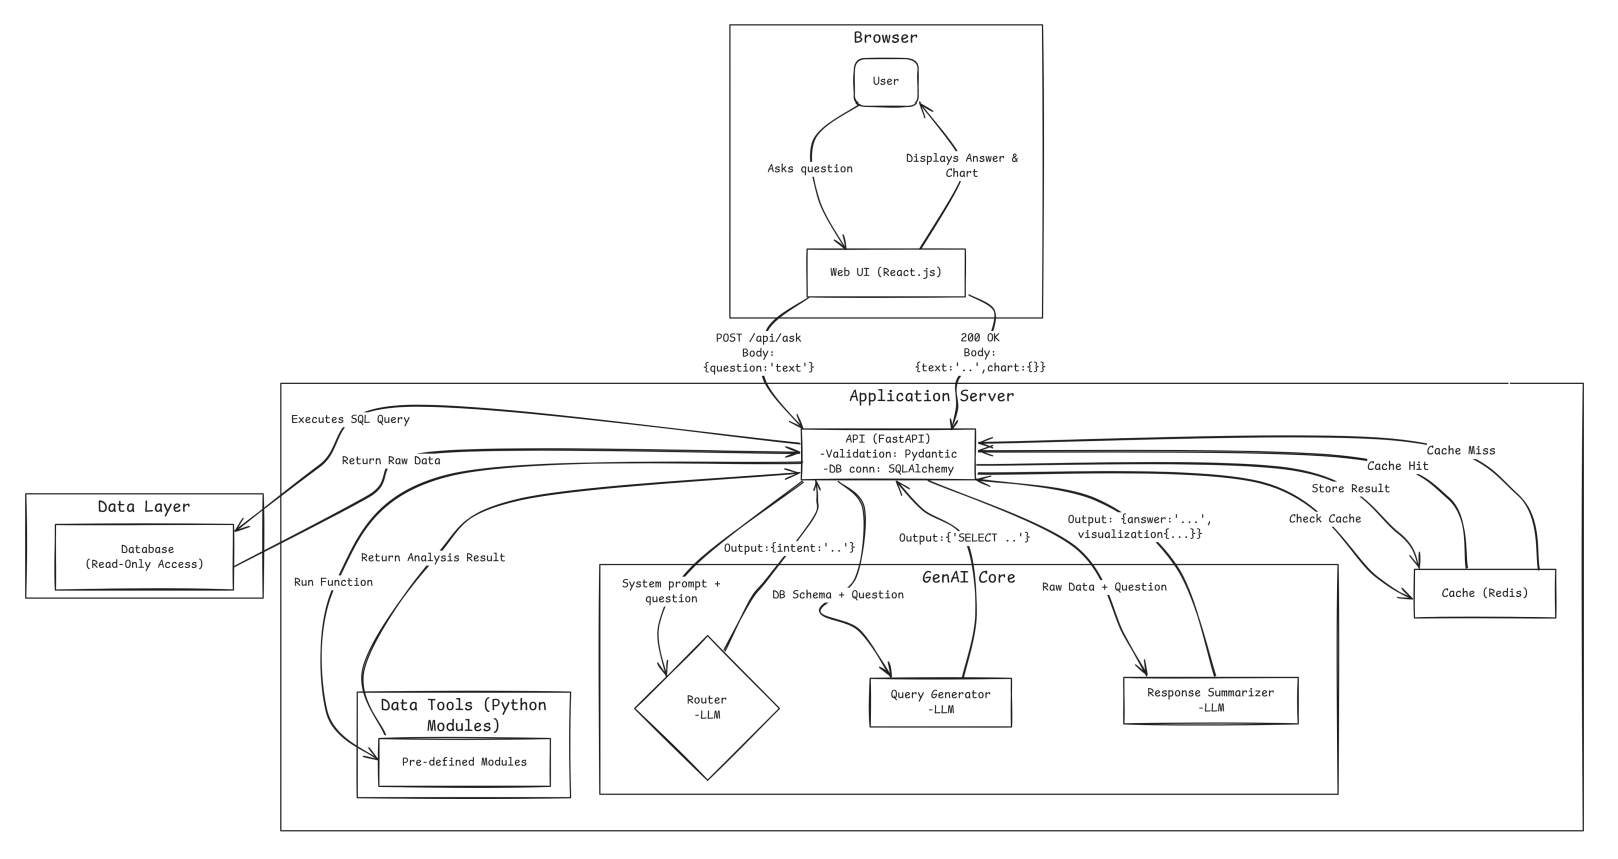
\includegraphics[width=0.95\textwidth]{arch_VDA.png}
\caption{Detailná architektúra systému s~komponentmi}
\end{figure}



\subsubsection{Backend komponenty}

\begin{table}[H]
\centering
\small
\begin{tabular}{lp{9cm}}
\toprule
\textbf{Komponent} & \textbf{Popis} \\
\midrule
\texttt{DatabaseManager} & Správa pripojenia k~PostgreSQL, vynucovanie READ-ONLY módu, získavanie schémy \\
\texttt{QueryGenerator} & LLM-based generovanie SQL dotazov pomocou GPT-4.1 \\
\texttt{ResponseSummarizer} & LLM-based sumarizácia výsledkov pomocou Gemini 2.5 Flash \\
\texttt{Router} & (TODO) Rozhodovanie medzi Data Tools a~Database queries \\
\texttt{RedisClient} & (TODO) Caching pre optimalizáciu opakovaných dotazov \\
\bottomrule
\end{tabular}
\caption{Backend komponenty a~ich zodpovednosti}
\end{table}

\subsubsection{API Endpoints}

\begin{table}[H]
\centering
\begin{tabular}{llp{6cm}}
\toprule
\textbf{Endpoint} & \textbf{Metóda} & \textbf{Popis} \\
\midrule
\texttt{/api/ask} & POST & Hlavný endpoint -- otázka $\rightarrow$ SQL $\rightarrow$ sumarizácia \\
\texttt{/api/generate-sql} & POST & Generovanie SQL bez vykonania \\
\texttt{/api/query-and-summarize} & POST & Vykonanie SQL a~sumarizácia \\
\texttt{/api/connect-database} & POST & Pripojenie k~databáze \\
\texttt{/api/disconnect-database} & POST & Odpojenie databázy \\
\texttt{/api/schema} & GET & Získanie schémy databázy \\
\bottomrule
\end{tabular}
\caption{REST API endpoints}
\end{table}

\subsubsection{Bezpečnostné mechanizmy}

Systém implementuje viacúrovňové zabezpečenie pre READ-ONLY prístup:

\begin{enumerate}
    \item \textbf{LLM Prompt} -- Systémový prompt zakazuje generovanie modifikačných príkazov
    \item \textbf{Regex validácia} -- Kontrola nebezpečných kľúčových slov (INSERT, UPDATE, DELETE, DROP...)
    \item \textbf{SQL Session} -- Nastavenie \texttt{SET TRANSACTION READ ONLY} na úrovni databázy
\end{enumerate}


\subsubsection{Frontend komponenty}

\begin{table}[H]
\centering
\begin{tabular}{lp{9cm}}
\toprule
\textbf{Komponent} & \textbf{Popis} \\
\midrule
\texttt{HomePage} & Hlavná stránka aplikácie, správa stavu pripojenia \\
\texttt{Chat} & Chat rozhranie pre komunikáciu s~analytikom \\
\texttt{SideBar} & Bočný panel s~ovládacími prvkami \\
\texttt{DatabaseModal} & Modal pre zadanie pripojovacích údajov k~databáze \\
\texttt{InputQuestion} & Vstupné pole pre zadávanie otázok \\
\texttt{UserMessage} & Zobrazenie správ v~chate \\
\bottomrule
\end{tabular}
\caption{React komponenty frontendu}
\end{table}

\clearpage

\section{Výber a~testovanie LLM modelov}

Pri návrhu systému bolo kľúčové rozhodnúť, ktoré veľké jazykové modely (LLM) použiť pre jednotlivé úlohy. Keďže systém vyžaduje dva odlišné typy spracovania -- generovanie SQL dotazov a~sumarizáciu výsledkov -- rozhodli sme sa pre špecializovaný prístup s~využitím rôznych modelov.

\subsection{Metodológia testovania}

Pre objektívne porovnanie výkonnosti LLM modelov sme vytvorili testovací skript, ktorý automatizovane vyhodnocoval schopnosti modelov riešiť SQL problémy. Ako zdroj testovacích úloh sme použili problémy z~platformy \textbf{HackerRank}, ktorá poskytuje široké spektrum SQL výziev rôznej obtiažnosti.

Testovací proces zahŕňal:
\begin{enumerate}
    \item \textbf{Kolekcia problémov} -- Výber 50+ SQL problémov z~HackerRank (easy, medium, hard)
    \item \textbf{Automatizované testovanie} -- Skript generoval dotazy pomocou každého modelu
    \item \textbf{Validácia výsledkov} -- Porovnanie vygenerovaných dotazov s~očakávanými výstupmi
    \item \textbf{Meranie metrík} -- Presnosť, čas odozvy, konzistencia výstupov
\end{enumerate}

\subsection{Porovnávané modely}

\begin{table}[H]
\centering
\begin{tabular}{ll}
\toprule
\textbf{Model} & \textbf{Poskytovateľ}  \\
\midrule
GPT-4.1 & OpenAI/Azure  \\
GPT-4o & OpenAI/Azure  \\
GPT-3.5-turbo & OpenAI/Azure  \\
Gemini 2.5 Flash & Google  \\
Gemini 2.5 Pro & Google  \\
Claude 4 Sonnet & Anthropic  \\
\bottomrule
\end{tabular}
\caption{Porovnávané LLM modely a~ich testované úlohy}
\end{table}

\subsection{Výsledky testovania -- SQL generácia}

Pre generovanie SQL dotazov sme testovali modely na nasledujúcich kritériách:

\begin{itemize}
    \item \textbf{Syntaktická správnosť} -- Percentuálna úspešnosť generovania validného SQL
    \item \textbf{Sémantická presnosť} -- Či dotaz vracia očakávané výsledky
    \item \textbf{Dodržiavanie pravidiel} -- Generovanie len READ-ONLY dotazov
    \item \textbf{Konzistencia} -- Stabilita výstupov pri opakovaných dotazoch
\end{itemize}

\textbf{GPT-4.1} dosiahol dobré výsledky v~syntaktickej aj sémantickej presnosti, pričom dosiahol aj dodržiavanie READ-ONLY pravidiel. Napriek vyššej latencii a mierne vyššej cene sme ho zvolili pre kritickú úlohu generovania SQL.

\subsection{Výsledky testovania -- Sumarizácia}

Pre sumarizáciu výsledkov sme hodnotili:

\begin{itemize}
    \item \textbf{Zrozumiteľnosť} -- Kvalita textu pre netechnických používateľov
    \item \textbf{Faktická správnosť} -- Presnosť interpretácie dát
    \item \textbf{Rýchlosť} -- Čas potrebný na generovanie odpovede
    \item \textbf{Cena} -- Náklady na API volania
\end{itemize}

\textbf{Gemini 2.5 Flash} ponúkol optimálny pomer kvality, rýchlosti a~ceny. Pri minimálnom rozdiele v~kvalite oproti drahším modelom poskytuje výrazne nižšiu latenciu, náklady a veľké kontextové okno.

\subsection{Záver výberu modelov}

Na základe testovania sme sa rozhodli pre kombináciu:

\begin{itemize}
    \item \textbf{GPT-4.1 (Azure)} pre generovanie SQL: dobrá presnosť a~spoľahlivosť pri dodržiavaní bezpečnostných pravidiel
    \item \textbf{Gemini 2.5 Flash (Vertex AI)} pre sumarizáciu: optimálny pomer veľkosť/cena/rýchlosť
\end{itemize}


\clearpage

\section{Použité technológie -- detailný prehľad}

\subsection{Backend technológie}

\begin{itemize}
    \item \textbf{Python 3.12+} -- Hlavný programovací jazyk
    \item \textbf{FastAPI} -- Moderný, asynchrónny webový framework
    \item \textbf{SQLAlchemy} -- ORM a~databázové pripojenie
    \item \textbf{OpenAI SDK} -- Klient pre LLM API (GPT-4.1, Gemini)
    \item \textbf{Pydantic} -- Validácia dát a~schémy
    \item \textbf{uv} -- Moderný Python package manager
\end{itemize}

\subsection{Frontend technológie}

\begin{itemize}
    \item \textbf{React} -- JavaScript knižnica pre UI
    \item \textbf{Vite} -- Rýchly build nástroj
    \item \textbf{Tailwind CSS} -- Utility-first CSS framework
    \item \textbf{Axios} -- HTTP klient pre API volania
\end{itemize}

\subsection{Infraštruktúra}

\begin{itemize}
    \item \textbf{Docker} -- Kontajnerizácia aplikácií
    \item \textbf{Docker Compose} -- Orchestrácia multi-kontajnerových aplikácií
    \item \textbf{Redis} -- In-memory cache
\end{itemize}

\subsection{AI/ML modely}

\begin{itemize}
    \item \textbf{GPT-4.1 (Azure)} -- Generovanie SQL dotazov
    \item \textbf{Gemini 2.5 Flash (Vertex AI)} -- Sumarizácia výsledkov
\end{itemize}

\clearpage
\section{Databázová vrstva}
Databázová vrstva predstavuje jednu zo základných súčastí navrhovanej aplikácie, keďže zabezpečuje ukladanie, spracovanie a poskytovanie dát pre ostatné komponenty systému. 

\subsection{Počiatočný návrh databázovej vrstvy}

Databázovú časť sme v úvodnej fáze vývoja navrhli tak, aby poskytovala dostatočný základ pre testovanie aplikácie a prácu s dátami. 
Použili sme kontajnerové riešenie, vďaka ktorému bolo možné databázu rýchlo spustiť a jednoducho integrovať do vývojového prostredia. 
Kontajner umožnil opakovateľné nasadenie rovnakého databázového prostredia, čo výrazne uľahčilo overovanie správnej funkcionality prepojenia s backendom.

Ako prvú databázu sme zvolili PostgreSQL, ktorá je stabilná a široko používaná relačná databáza. 
Štruktúra databázy vychádzala z verejne dostupného datasetu z platformy  \textbf{Kaggle}, ktorý obsahuje údaje o správaní zákazníkov v e-commerce prostredí.\newline 

Pred samotným použitím sme dataset upravili tak, aby bolo možné dáta efektívne využívať počas vývoja a testovania aplikácie. 
Konkrétne sme vykonali nasledujúce úpravy:

\begin{itemize}
    \item odstránili sme neúplné záznamy, ktoré by mohli negatívne ovplyvniť testovanie,
    \item zjednotili sme dátové typy pre zjednodušenie importu a spracovania dát,
    \item pripravili sme dataset na automatický import do databázy.\newline
\end{itemize}

\noindent 
V inicializačnom SQL skripte sme vytvorili tabuľku \texttt{events}, ktorá obsahuje kľúčové stĺpce:

\begin{itemize}
    \item \texttt{event\_id} – jedinečný identifikátor udalosti,
    \item \texttt{event\_time} – čas vzniku udalosti,
    \item \texttt{event\_type} – typ udalosti,
    \item \texttt{product\_id}, \texttt{category\_id},
    \item \texttt{category\_code}, \texttt{brand},
    \item \texttt{price}, \texttt{user\_id},
    \item \texttt{user\_session}.\newline
\end{itemize}

Súčasťou skriptu bolo aj vytvorenie indexov pre rýchle vyhľadávanie podľa času udalosti, typu udalosti, produktu a používateľa. 
Tento prístup umožňuje efektívnu prácu s databázou aj pri väčších objemoch dát. 
Dáta sa automaticky načítavali zo súboru CSV pri štarte databázového kontajnera, takže boli hneď pripravené na testovanie.
Takto pripravená databáza umožnila overiť správnu komunikáciu backendu s databázou, testovať základné operácie s dátami a kontrolovať korektnosť ich spracovania. 
Napriek tomu, že nešlo o finálnu databázovú vrstvu, predstavovala vhodný základ pre ďalší vývoj aplikácie.\clearpage
V tejto fáze bola databáza súčasťou rovnakého projektu \texttt{Docker Compose} ako backend a frontend, čo umožňovalo spúšťanie všetkých služieb naraz a výrazne zjednodušovalo integráciu a úvodné testovanie aplikácie.

S postupujúcim vývojom aplikácie sme sa rozhodli databázu oddeliť do samostatného súboru \texttt{Docker Compose}. 
Toto riešenie umožňuje databázu spúšťať a spravovať nezávisle od backendu a frontendu, zjednodušuje jej samostatné testovanie a poskytuje väčšiu kontrolu nad konfiguráciou databázového prostredia, napríklad pri zmene verzie databázy. 
Oddelenie databázy zároveň vytvára priestor pre ďalšie úpravy a plánované rozšírenia aplikácie o podporu rôznych typov databáz.

\subsection{Pripájanie na databázu}

Po vytvorení a inicializácii databázového prostredia bolo ďalším krokom návrh a implementácia aplikačnej vrstvy, ktorá umožňuje backendu dynamicky sa pripájať k databáze.

Databázový konektor bol navrhnutý ako samostatná logická súčasť backendu, ktorá sprostredkúva komunikáciu medzi aplikáciou a databázou PostgreSQL. 
Cieľom bolo umožniť flexibilné pripojenie k rôznym databázovým inštanciám bez nutnosti meniť kód aplikácie.
Hlavné vlastnosti konektora:

\begin{itemize}
    \item bol implementovaný ako modul vo FastAPI,
    \item využíva štandardné PostgreSQL knižnice na nadväzovanie spojenia,
    \item podporuje dynamické vytváranie pripojenia na základe vstupov používateľa,
    \item uchováva informáciu o aktívnom pripojení počas behu aplikácie.
\end{itemize}

\subsubsection{API endpointy pre správu pripojenia}

Na ovládanie databázového spojenia sme vytvorili dva samostatné API endpointy:

\begin{enumerate}
    \item Endpoint na pripojenie k databáze
    \begin{itemize}
        \item umožňuje používateľovi nadviazať spojenie s databázou,
        \item prijíma prihlasovacie údaje v tele požiadavky,
        \item po úspešnom pripojení vracia potvrdenie o nadviazaní spojenia.
    \end{itemize}
    \item Endpoint na odpojenie od databázy
    \begin{itemize}
        \item slúži na bezpečné ukončenie aktívneho pripojenia,
        \item používateľ ho aktivuje jednoduchým kliknutím (alebo volaním endpointu),
        \item zabezpečuje uvoľnenie zdrojov na strane backendu.\newline
    \end{itemize}
\end{enumerate}
\clearpage
\noindent
Pri vytváraní spojenia používateľ zadáva nasledujúce parametre:

\begin{itemize}
    \item Host – adresa databázového servera,
    \item User – meno databázového používateľa,
    \item Password – prístupové heslo k databáze,
    \item Database name – meno cieľovej databázy,
    \item Port – port, na ktorom databáza počúva.
\end{itemize}

\noindent
Tieto údaje sú zasielané backendu, ktorý ich následne spracuje.
Na základe zadaných údajov aplikácia automaticky vytvorí tzv. connection string.
Tento reťazec sa následne použije na inicializáciu spojenia s databázou prostredníctvom databázovej knižnice.

\subsubsection*{Podporované typy pripojenia}

Aplikácia umožňuje pripojenie na dva typy databázových prostredí:
\begin{itemize}
    \item Lokálnu databázu
    \begin{itemize}
        \item bežiacu priamo na počítači vývojára alebo serveri,
        \item vhodnú najmä na vývoj a testovanie.
    \end{itemize}
    \item Databázu spustenú v Docker kontajneri
    \begin{itemize}
        \item bežiacu na pozadí ako samostatná služba,
        \item prístupnú cez názov kontajnera alebo localhost,
        \item využívanú najmä pri integrácii s ostatnými službami v Docker Compose.
    \end{itemize}
\end{itemize}

\subsubsection*{Odpojenie databázy}

Proces odpojenia je riešený jednoducho:
\begin{itemize}
    \item používateľ aktivuje endpoint na odpojenie,
    \item backend uzavrie aktívne spojenie,
    \item systém uvoľní pridelené zdroje,
    \item aplikácia prejde do stavu „nepripojená“.
    \item Tento mechanizmus zabraňuje zbytočnému držaniu otvorených spojení.
\end{itemize}

\noindent
Po úspešnom pripojení k databáze aplikácia umožňuje:
\begin{itemize}
    \item načítať zoznam dostupných tabuliek,
    \item zobraziť stĺpce vybranej tabuľky,
    \item vypísať názvy stĺpcov spolu s ich dátovými typmi.
\end{itemize}

\clearpage
\section{Frontendová časť aplikácie}

\subsubsection{Štruktúra projektu}

Frontendová časť aplikácie je implementovaná pomocou knižnice React v kombinácii s nástrojom Tailwind. Projekt je rozdelený do modulov, aby bol prehľadný a komponenty sa dali ľahko znovu použiť. Komponenty sú navrhnuté tak, aby boli čo najviac nezávislé a komunikovali medzi sebou prostredníctvom vlastností (props).

Adresárová štruktúra projektu je nasledovná:

\begin{itemize}
    \item \texttt{components/} - Komponenty, ktoré tvoria používateľské rozhranie, napríklad chat, bočný panel, modálne okná a vstupné polia.
    \item \texttt{hooks/} - Vlastné React hooky, ktoré riešia logiku aplikácie, napríklad pripojenie k databáze.
    \item \texttt{services/} - Funkcie na komunikáciu s backendom.
    \item \texttt{pages/} - Komponenty pre hlavné stránky aplikácie.
    \item \texttt{assets/} - Obrázky, ikony a iné statické súbory.
    \item \texttt{api/} - Nastavenie HTTP klienta pre volania na backend.
\end{itemize}

\subsubsection{Správa stavu aplikácie}

Správa stavu aplikácie je realizovaná pomocou vstavaných React hookov \texttt{useState}, \texttt{useEffect} a \texttt{useRef}.

Stavy sú spravované lokálne v jednotlivých komponentoch, napríklad:
\begin{itemize}
    \item otvorenie a zatvorenie modálneho okna pre databázu,
    \item stav načítavania počas pripájania databázy,
    \item vstupné hodnoty formulárových polí,
    \item priebeh komunikácie v chatovom rozhraní.
\end{itemize}

\subsubsection{Vlastné React hooky}

Vo fronte je použitý vlastný React hook \texttt{useDatabase}, ktorý sa stará o pripojenie a odpojenie databázy. Komponenty ho môžu použiť bez toho, aby sa museli starať o detaily HTTP komunikácie.  

Hook \texttt{useDatabase}:
\begin{itemize}
    \item pripája a odpojuje databázu cez backend,
    \item sleduje, či sa práve načítava (\texttt{loading}),
    \item uchováva a zobrazuje chyby (\texttt{error}),
\end{itemize}


\subsection{Komunikácia s backendom}

Frontendová aplikácia komunikuje s backendom prostredníctvom HTTP požiadaviek. 
Táto komunikácia zabezpečuje pripojenie a odpojenie databázy, ako aj odosielanie otázok používateľa a prijímanie odpovedí od systému. Frontend odosiela požiadavky na backend vo formáte JSON a backend vracia odpovede v rovnakom formáte.

\subsubsection{Správa API volaní pomocou Axios}

Pre komunikáciu s backendom je použitá knižnica \textbf{Axios}. 
V projekte je vytvorený jeden centrálny Axios klient, ktorý obsahuje základnú konfiguráciu, ako je adresa backendového servera a hlavičky požiadaviek.

\begin{lstlisting}[caption={Základná konfigurácia Axios klienta}]
import axios from "axios";

const api = axios.create({
  baseURL: import.meta.env.VITE_API_BASE_URL || "http://localhost:8000",
  headers: {
    "Content-Type": "application/json",
  },
});

export default api;
\end{lstlisting}

Na základe tohto klienta sú vytvorené servisné funkcie, ktoré reprezentujú jednotlivé API volania.

\begin{lstlisting}[caption={Servisné funkcie pre komunikáciu s backendom}]
import api from "./api";

export const connectDatabase = async (data) => {
  const response = await api.post("/api/connect-database", data);
  return response.data;
};

export const disconnectDatabase = async () => {
  const response = await api.post("/api/disconnect-database");
  return response.data;
};

export const askQuestion = async (question) => {
  const response = await api.post("/api/ask", {
    question,
  });
  return response.data;
};
\end{lstlisting}

\subsection{Používateľské rozhranie}

Frontendová aplikácia má jednoduché a prehľadné rozhranie, ktoré umožňuje používateľovi komunikovať so systémom a spravovať pripojenie k databáze.

\subsubsection{Rozloženie aplikácie}

Hlavná stránka je rozdelená na dve časti:

\begin{itemize}
    \item \textbf{Bočný panel (Sidebar)} - obsahuje tlačidlá na otvorenie modálu pre pripojenie k databáze a ďalšie ovládacie prvky.
    \item \textbf{Hlavný obsah (Chat)} - zobrazujú sa správy medzi používateľom a systémom.
\end{itemize}

\begin{figure}[H]
\centering
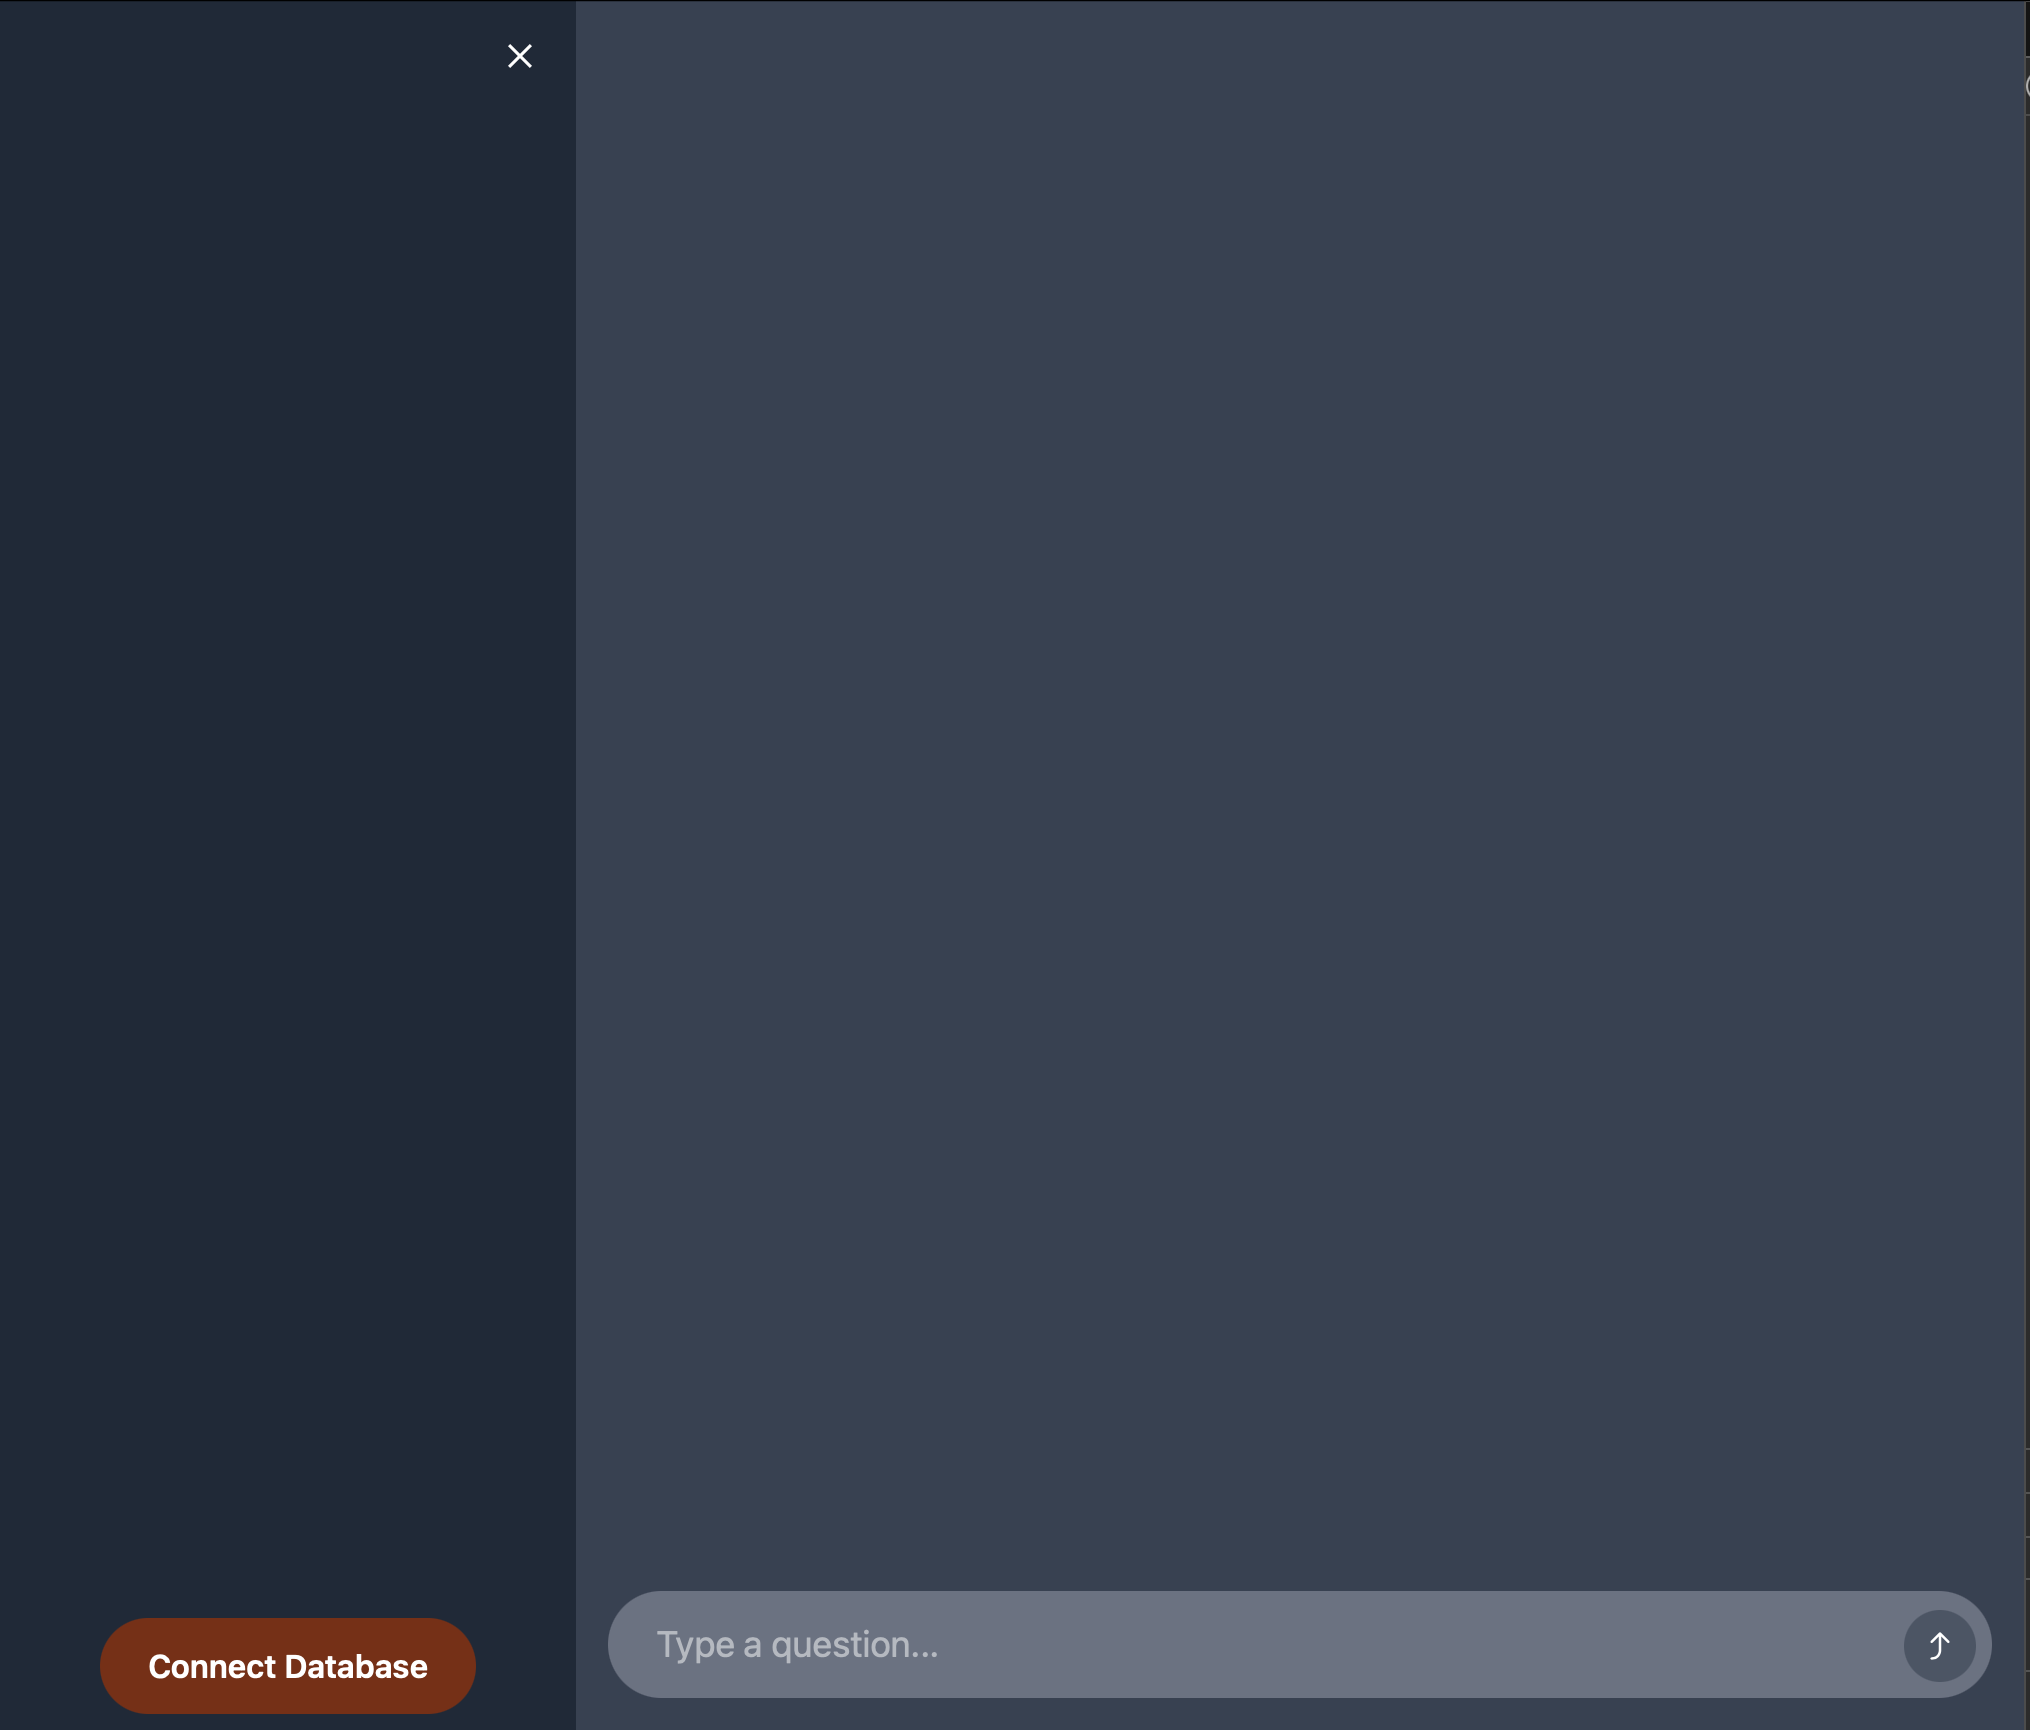
\includegraphics[width=0.95\textwidth]{frontend_layout.png}
\caption{Ukážka rozloženia frontendovej aplikácie}
\end{figure}
\clearpage
\subsubsection{Chatové rozhranie}

Chat pozostáva z oblasti správ a vstupného poľa na zadávanie otázok. Používateľ môže zadávať otázky, ktoré sú posielané systému, a výsledky sa zobrazujú v chronologickom poradí.


\begin{figure}[H]
\centering
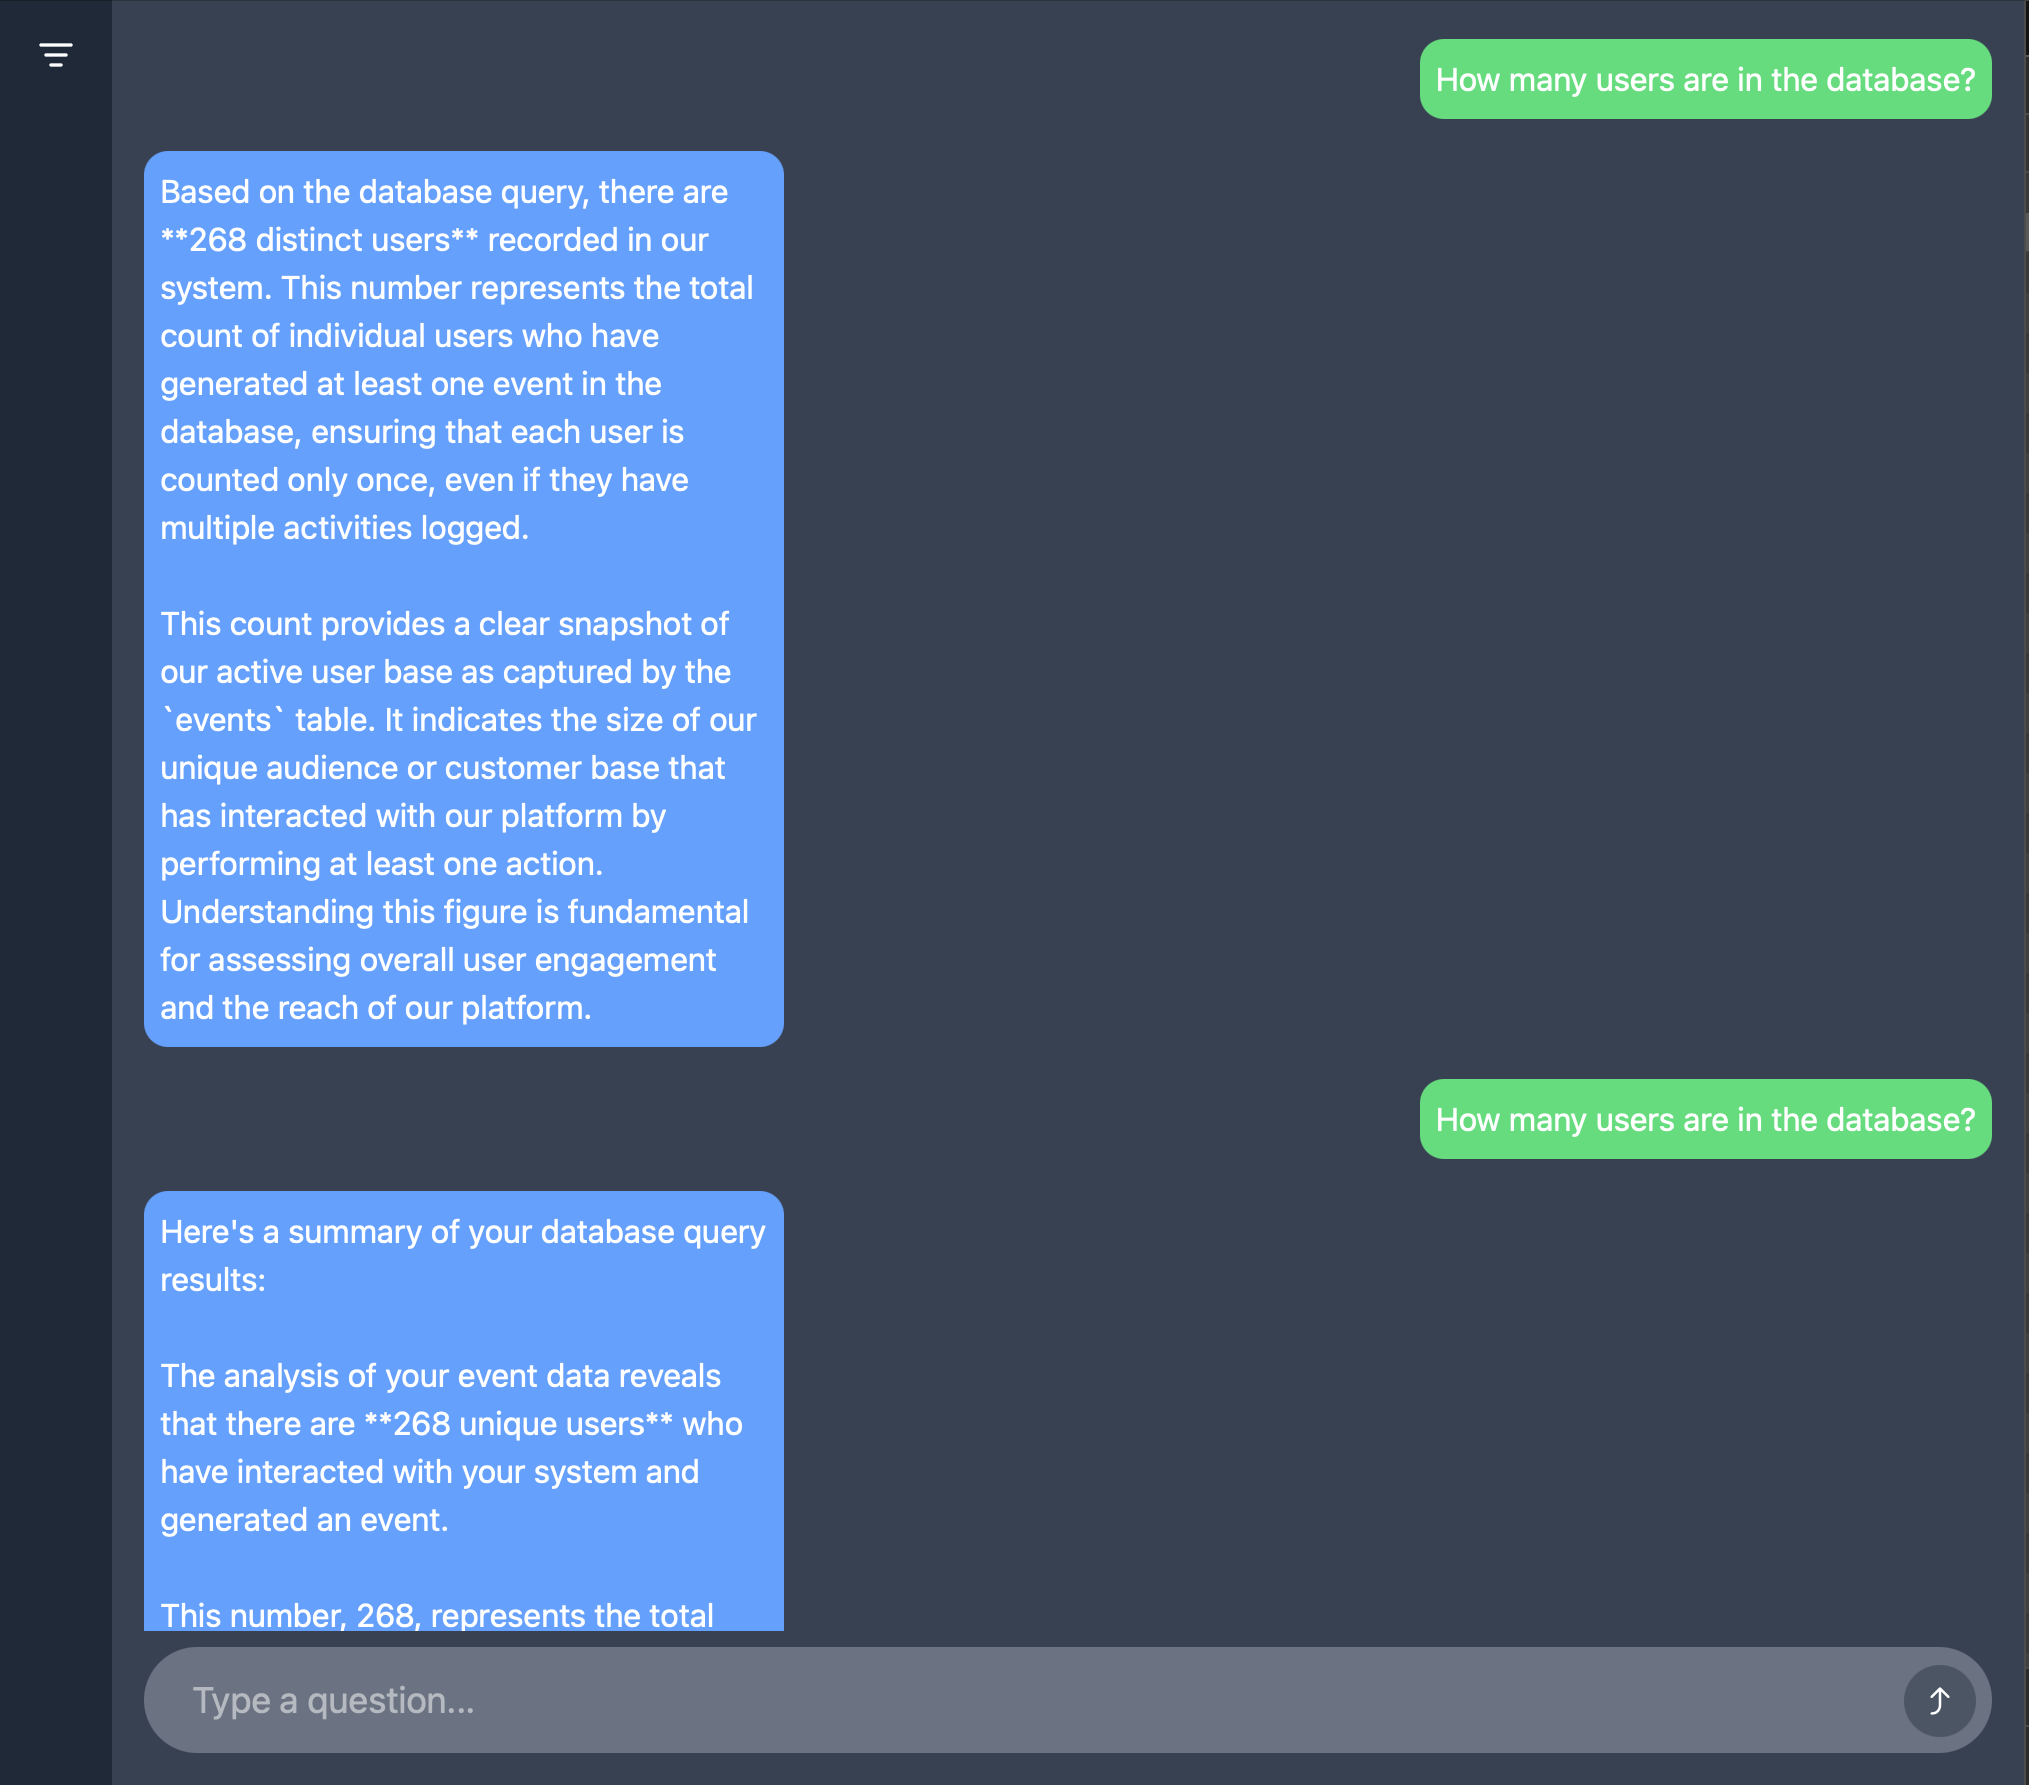
\includegraphics[width=0.8\textwidth]{chat_example.png}
\caption{Ukážka chatového rozhrania}
\end{figure}

\subsubsection{Správa pripojenia k databáze}

Používateľ môže databázu pripojiť alebo odpojiť pomocou tlačidla v bočnom paneli.  
Stav pripojenia sa vizuálne zobrazuje priamo na tlačidle:
\begin{itemize}
    \item \textbf{Connect Database} - databáza nie je pripojená,
    \item \textbf{Disconnect Database} - databáza je pripojená.
\end{itemize}


\begin{figure}[H]
\centering
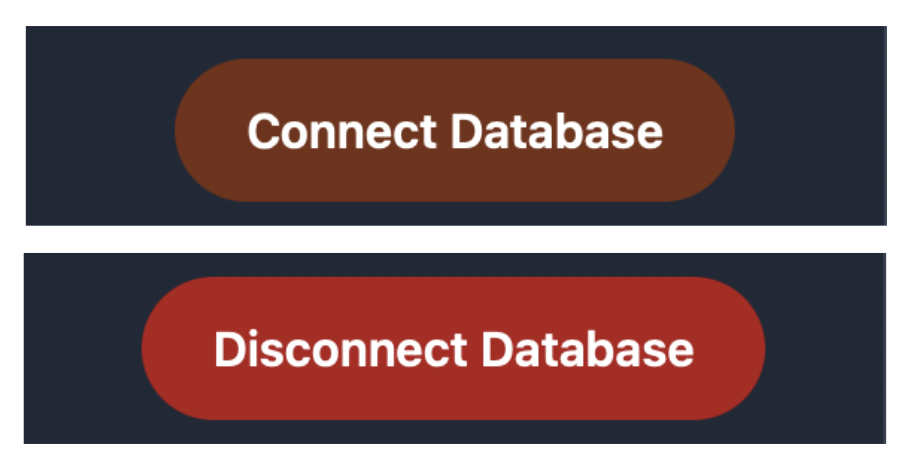
\includegraphics[width=0.45\textwidth]{database_button.png}
\caption{Stav pripojenia k databáze zobrazený na tlačidle}
\end{figure}

\subsubsection{Modálne okno}

Modálne okno slúži na zadanie údajov potrebných na pripojenie k databáze, ako sú hostiteľ, port, používateľské meno, heslo a názov databázy. Počas pripájania sa používateľovi zobrazuje stav \textbf{Connecting...}, aby vedel, že sa proces práve vykonáva. V prípade chyby sa zobrazí chybová hláška, ktorá informuje o neúspešnom pripojení.


\begin{figure}[H]
\centering
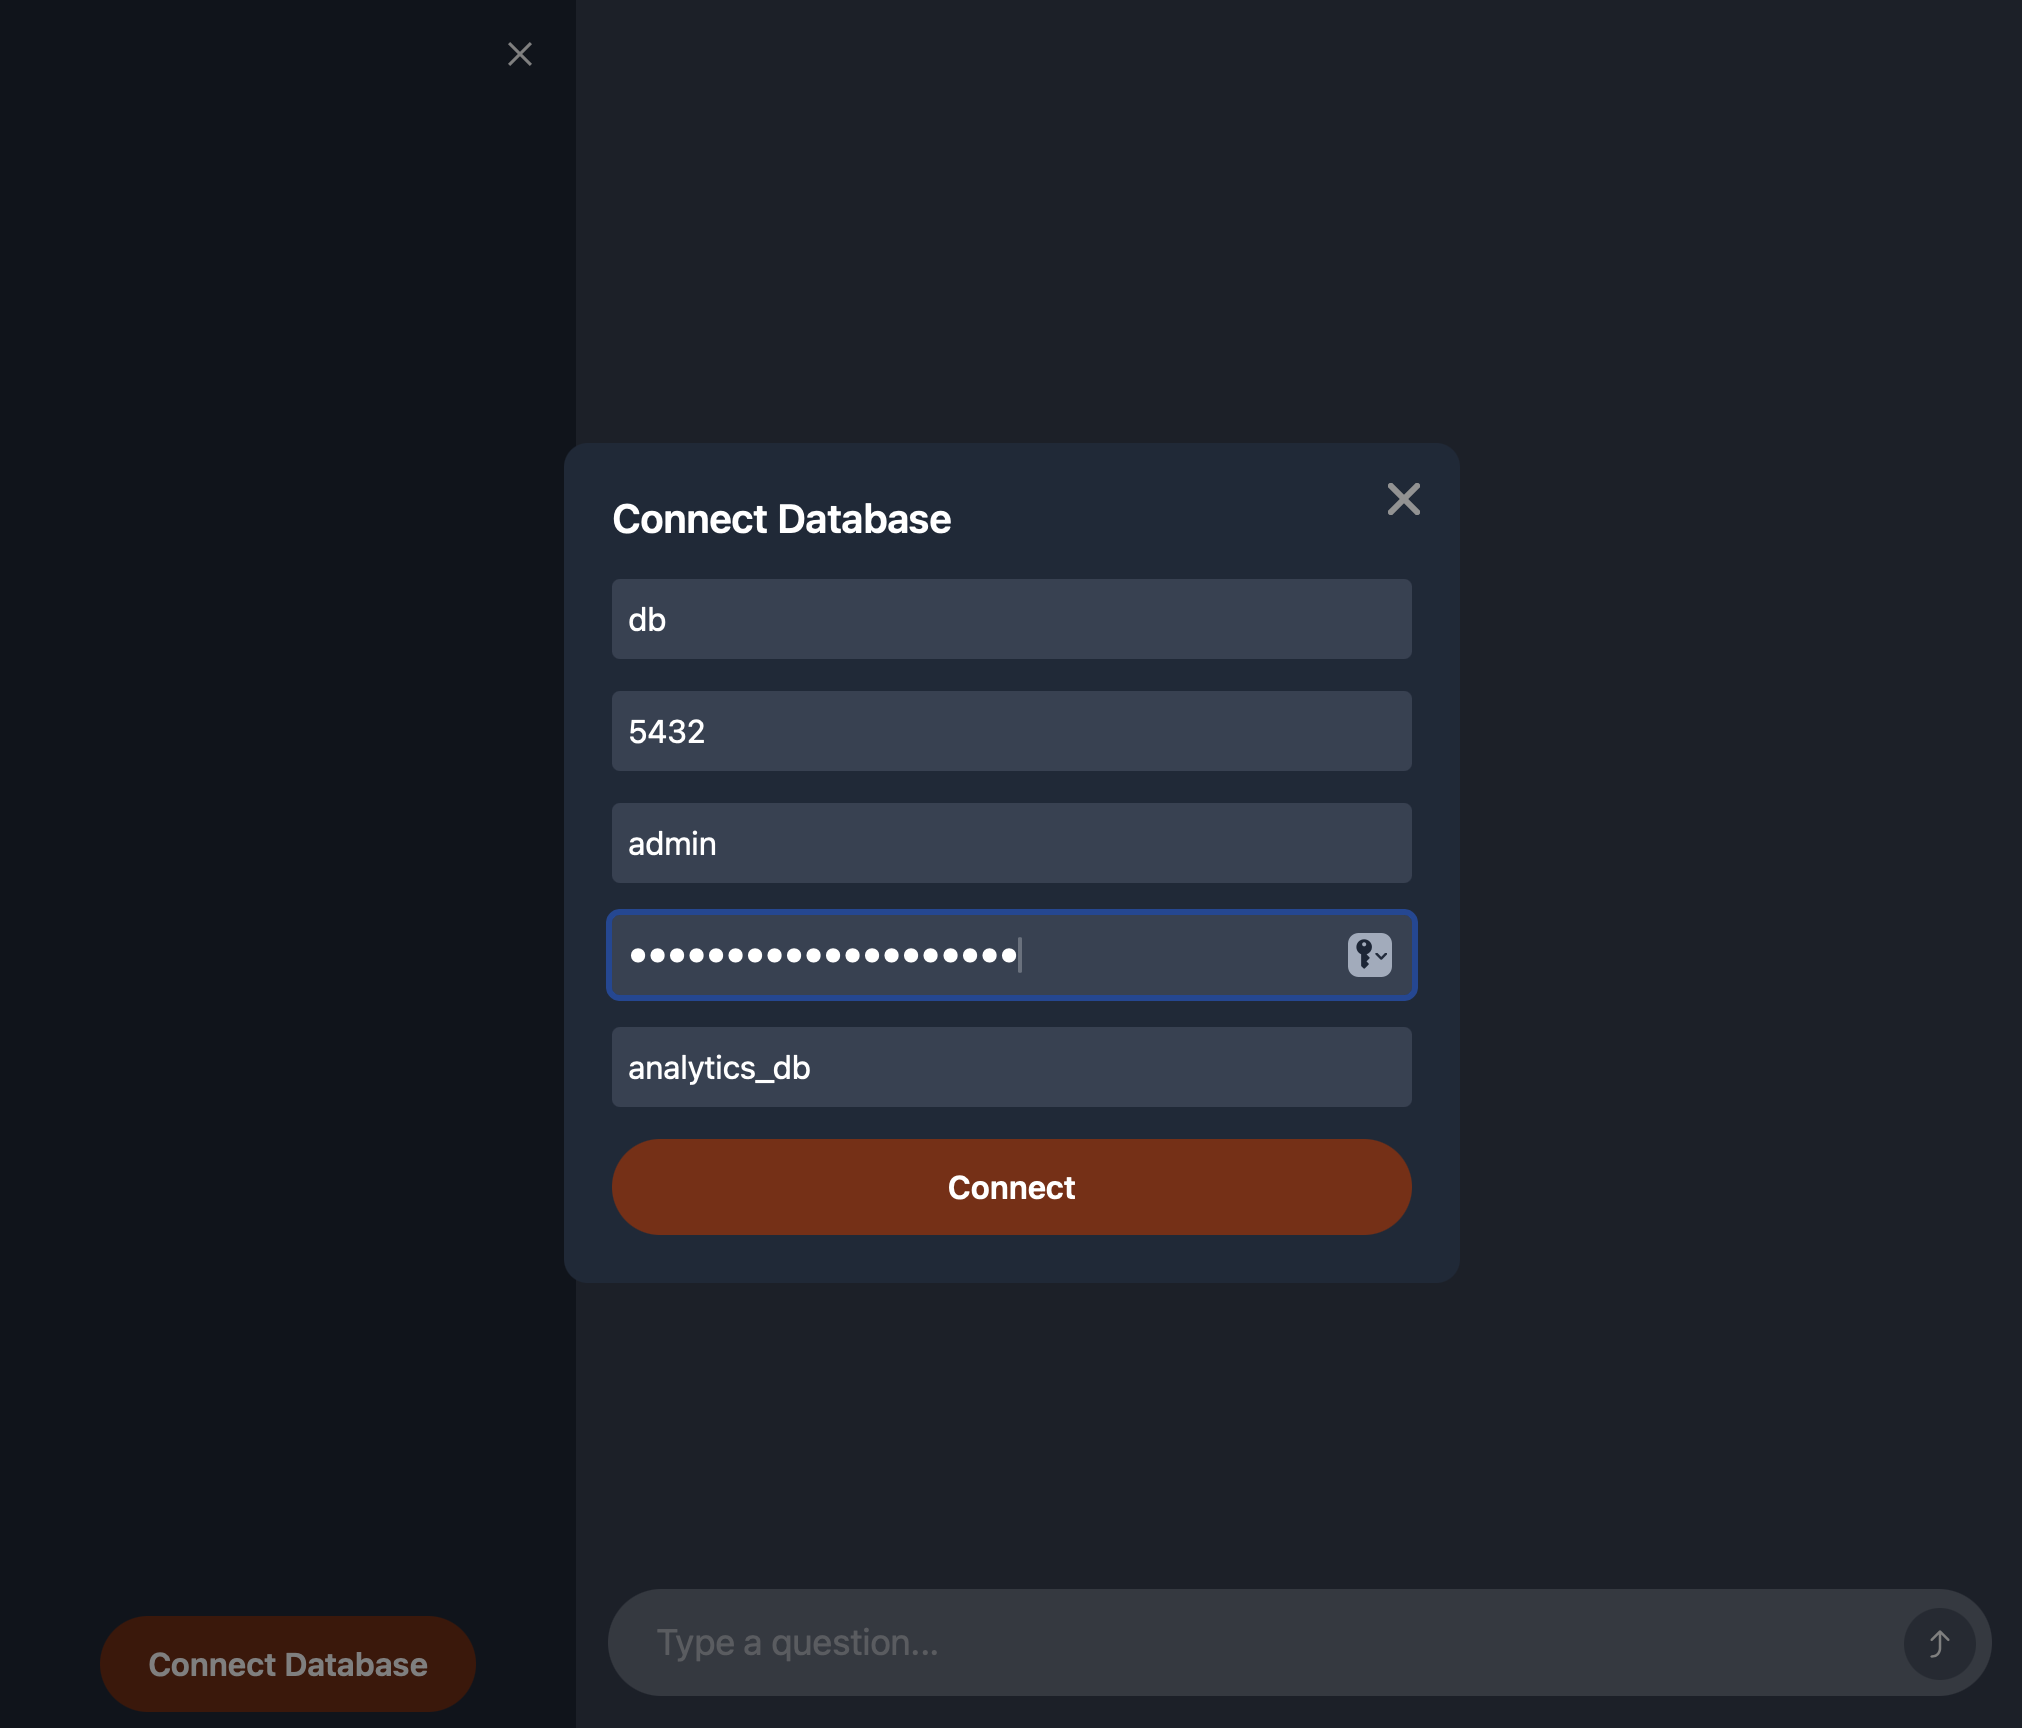
\includegraphics[width=0.9\textwidth]{database_modal.png}
\caption{Ukážka modálneho okna pre pripojenie databázy}
\end{figure}


\clearpage
\section*{Použitie nástrojov umelej inteligencie}

Pri vypracovaní projektu sme využili nasledujúce AI nástroje ako podporné prostriedky:

\begin{itemize}
    \item \textbf{Claude Opus 4.5 (Anthropic, 2025):} Využitý pri návrhu architektúry systému, code review a~optimalizácii kódu. Pomáhal s~formuláciou systémových promptov pre LLM komponenty.
\end{itemize}
\begin{itemize}
    \item \textbf{Claude Sonnet 4.5 (Anthropic, 2025):} Využitý pri návrhu architektúry systému, code review a~optimalizácii kódu. Pomáhal s~formuláciou systémových promptov pre LLM komponenty.
\end{itemize}
\begin{itemize}
    \item \textbf{GPT-4.1 (OpenAI/Azure, 2025):} Integrovaný priamo v~systéme ako Query Generator pre transformáciu prirodzeného jazyka na SQL dotazy.
\end{itemize}

\begin{itemize}
    \item \textbf{Gemini 2.5 Flash (Google, 2025):} Integrovaný v~systéme ako Response Summarizer pre generovanie zrozumiteľných textových sumarizácií výsledkov dotazov.
\end{itemize}


\clearpage

\section*{Zdroje}

\begin{enumerate}
    \item FastAPI Documentation. (2025). \textit{FastAPI - Modern, Fast Web Framework}. \\
    \url{https://fastapi.tiangolo.com/}
    
    \item React Documentation. (2025). \textit{React - A JavaScript Library for Building User Interfaces}. \\
    \url{https://react.dev/}
    
    \item OpenAI. (2025). \textit{GPT-4 API Documentation}. \\
    \url{https://platform.openai.com/docs/}
    
    \item Google Cloud. (2025). \textit{Vertex AI - Gemini API}. \\
    \url{https://cloud.google.com/vertex-ai/docs/generative-ai/}
    
    \item PostgreSQL Global Development Group. (2025). \textit{PostgreSQL Documentation}. \\
    \url{https://www.postgresql.org/docs/}
    
    \item SQLAlchemy Documentation. (2025). \textit{SQLAlchemy - The Database Toolkit for Python}. \\
    \url{https://docs.sqlalchemy.org/}
    
    \item Docker Documentation. (2025). \textit{Docker Docs}. \\
    \url{https://docs.docker.com/}
    
    \item Redis Documentation. (2025). \textit{Redis Documentation}. \\
    \url{https://redis.io/documentation}

    \item Medium (2023). \textit{Building Fast and Robust APIs with FastAPI and SQL Databases}. \\
    \url{https://medium.com/towards-data-engineering/fastapi-with-sql-1c7852ccbf21}
    
    \item Budibase. (2023). \textit{How to Integrate Multiple Databases}. \\
    \url{https://budibase.com/blog/data/how-to-integrate-multiple-databases/}
    
    \item Vite Documentation. (2025). \textit{Vite - Next Generation Frontend Tooling}. \\
    \url{https://vitejs.dev/}
    
    \item Tailwind CSS Documentation. (2025). \textit{Tailwind CSS - A Utility-First CSS Framework}. \\
    \url{https://tailwindcss.com/docs}
    
    \item Axios Documentation. (2025). \textit{Axios - Promise Based HTTP Client}. \\
    \url{https://axios-http.com/docs/intro}
    
    \item React Hooks Documentation. (2025). \textit{React Hooks - State and Lifecycle in Functional Components}. \\
    \url{https://react.dev/reference/react/hooks}
    
    \item Brown, T., et al. (2020). \textit{Language Models are Few-Shot Learners}. \\
    \url{https://arxiv.org/abs/2005.14165}
    
    \item Rajkumar, N., et al. (2022). \textit{Evaluating the Text-to-SQL Capabilities of Large Language Models}. \\
    \url{https://arxiv.org/abs/2204.00498}
    
    \item Pourreza, M., \& Rafiei, D. (2024). \textit{DIN-SQL: Decomposed In-Context Learning of Text-to-SQL}. \\
    \url{https://arxiv.org/abs/2304.11015}
\end{enumerate}

\end{document}